\section{Evaluation}\label{sec:eval}

\subsection{Headline Numbers}
Table~\ref{tab:headline} summarizes the hero
$(\mathrm{workload}, \mathrm{threads})$ cells from the phase-10 cert
(\texttt{phase10-xbabe1-certified}, git SHA \texttt{7c10410},
\texttt{ratio.csv} hash
\texttt{88aaab91...}). Throughput is operations per second computed as
the median of five repetitions; ratios are RedlineDB qps divided by
SQLite qps.

\begin{table}[t]
\centering
\caption{Phase-10 headline qps and Redline/SQLite ratio at strict
durability, with the phase-9 wave-7 ratio for reference (median of
five reps; xbabe1 128-vCPU host)}
\label{tab:headline}
\renewcommand{\arraystretch}{1.05}
\setlength{\tabcolsep}{3pt}
\footnotesize
\begin{tabular}{@{}lrrrrr@{}}
\toprule
\textbf{Workload} & \textbf{Thr.} & \textbf{R-qps} & \textbf{S-qps}
& \textbf{P-10 Ratio} & \textbf{P-9 Ratio} \\
\midrule
point-read-pk        & 64 & 121{,}268 & 122{,}221 & 0.99$\times$ & 0.99$\times$ \\
writers-disjoint     & 64 &  1{,}256  &      79  & \textbf{15.89$\times$} & 8.32$\times$ \\
mixed95-r5w          & 64 & 24{,}763  & 1{,}680  & \textbf{14.74$\times$} & 7.92$\times$ \\
mixed80-r20w         & 64 &  6{,}154  &     405  & \textbf{15.21$\times$} & 8.01$\times$ \\
mixed50-r50w         & 64 &  2{,}483  &     160  & \textbf{15.55$\times$} & 7.90$\times$ \\
hot-row-update       & 64 &       35  &      79  & 0.44$\times$ & 0.21$\times$ \\
secondary-index-range & 64 & 5{,}598  & 117{,}088 & 0.048$\times$ & 0.012$\times$ \\
secondary-index-read & 64 & 16{,}245  & 121{,}030 & 0.13$\times$ & n/a \\
\bottomrule
\end{tabular}
\end{table}

The phase-10 cert preserves the parity story at the 64-thread
point-read peak (0.99$\times$, identical to phase-9) and roughly
\textbf{doubles} the four contended-write headlines. \texttt{writers-disjoint}
moves from 8.32$\times$ to 15.89$\times$; the three mixed cells move
from 7.9--8.0$\times$ into the 14.7--15.6$\times$ band. The two
contention-bound losers also improve: \texttt{hot-row-update}
doubles (0.21$\rightarrow$0.44$\times$) and
\texttt{secondary-index-range} improves 4$\times$
(0.012$\rightarrow$0.048$\times$), though both still trail SQLite.
SQLite's p99 in the contended-write cells remains in the multi-second
range while RedlineDB's p99 stays inside the hundred-millisecond band.

The improvement is attributable to the phase-10 kernel changes that
landed under the same parallel-agent fusion discipline as the
phase-9 waves: per-entry index MVCC tags
($(\texttt{create\_tx}, \texttt{delete\_tx})$) replaced the boolean
\texttt{dead} flag, eliminating a write barrier that the previous
B-tree maintained on every mutation; the
\texttt{CommitOutcome::MaybeCommitted} protocol let the SQL layer
remove its post-commit index-undo log entirely (mutations now ride
kernel index visibility, not an SQL-side write-twice path); and
group-commit telemetry surfaced the existing batch coalescing that
phase-9 carried but never measured.

The two remaining losses in the table are the honest
counter-evidence: \texttt{hot-row-update} (every contender targets
a single row) still trails because RedlineDB's row-lock manager
serializes every write through one queue while SQLite's WAL writer
batches updates and amortizes the fsync; \texttt{secondary-index-range}
trails because the index cursor still lacks the prefetch path
SQLite ships. Both gaps are addressable engineering items
(Section~\ref{sec:discussion}).

\subsection{Throughput Scaling}
Figure~\ref{fig:thruput} shows throughput on a log-y axis as a
function of thread count for five representative workloads, RedlineDB
solid and SQLite dashed. The mixed and writers-disjoint workloads
diverge near 8 threads and the gap widens through 64; the
point-read-pk lines converge at the top end as both engines saturate.

\begin{figure}[t]
\centering
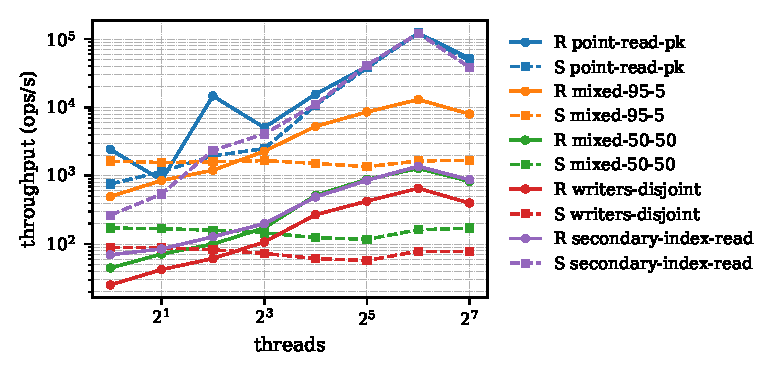
\includegraphics[width=\columnwidth]{figs/fig1_throughput_scaling.eps}
\caption{Throughput vs threads (log-y) for five representative
workloads. RedlineDB solid, SQLite dashed.}
\label{fig:thruput}
\end{figure}

\subsection{p99 Latency}
Figure~\ref{fig:p99} shows the corresponding p99 latency. SQLite's
mixed-workload p99 climbs into the multi-second range past 32
threads as contenders queue on the single writer; RedlineDB stays in
the hundred-millisecond band. On point-read-pk the two engines track
each other.

\begin{figure}[t]
\centering
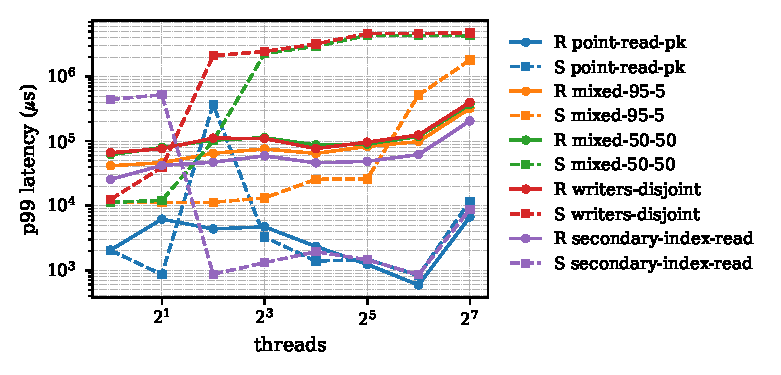
\includegraphics[width=\columnwidth]{figs/fig2_latency_p99.eps}
\caption{p99 latency vs threads for the same five workloads.}
\label{fig:p99}
\end{figure}

\subsection{Ratio Bars}
Figure~\ref{fig:ratio} renders the same data as Redline/SQLite ratios
at $\{1, 8, 32, 64, 128\}$ threads. Bars at or above 4$\times$ are
the wins; bars below 1$\times$ are the losses. The mixed and
writers-disjoint workloads dominate the upper region; hot-row-update
and secondary-index-range live at the bottom.

\begin{figure}[t]
\centering
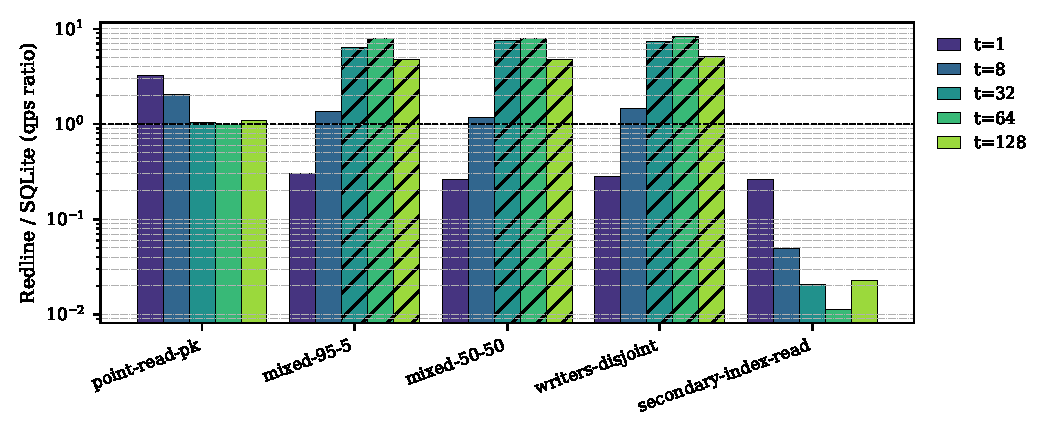
\includegraphics[width=\columnwidth]{figs/fig3_ratio_bars.eps}
\caption{Redline/SQLite throughput ratio per (workload, thread).}
\label{fig:ratio}
\end{figure}

\subsection{Scaling Efficiency}
Figure~\ref{fig:eff} plots scaling efficiency
($\mathrm{qps}(N)/\mathrm{qps}(1)$) against an ideal linear line.
RedlineDB tracks within a factor of two of ideal on point-reads
through 32 threads. SQLite's mixed-workload curve flattens almost
immediately, because the single-writer WAL caps the achievable
parallelism regardless of how many threads the host offers.

\begin{figure}[t]
\centering
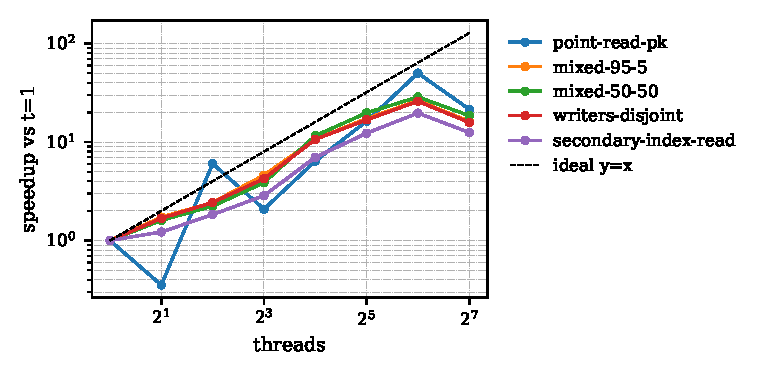
\includegraphics[width=\columnwidth]{figs/fig4_scaling_efficiency.eps}
\caption{Scaling efficiency vs ideal linear scaling.}
\label{fig:eff}
\end{figure}

\subsection{Recovery and Failpoint Matrix}
Figure~\ref{fig:recovery} summarizes the deterministic-crash
certification: 36/36 recovery cases pass, 24/24 failpoint cases
pass, and the oracle observed 0 lost-acked-commits across all of
them. The fdatasync passthrough counter, surfaced into every
benchmark row via the WAL coordinator, is what lets us assert the
durability story is the one we measured rather than the one we hoped
for.

\begin{figure}[t]
\centering
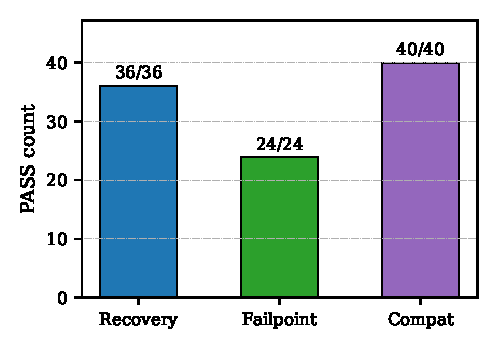
\includegraphics[width=\columnwidth]{figs/fig5_recovery_failpoint.eps}
\caption{Recovery matrix (36/36) and failpoint matrix (24/24) pass
counts.}
\label{fig:recovery}
\end{figure}

\subsection{Phase 10 Feature Lanes}
Figures~\ref{fig:json}, \ref{fig:vector}, and
\ref{fig:groupcommit} are generated from the phase-10 cert-v3 lane.
The JSON lane separates path extraction from path mutation, the vector
lane reports flat exact search alongside HNSW and DiskANN-style
approximate search, and the group-commit lane plots the WAL
coordinator's records-per-fdatasync batch histogram under a tiny
commit storm. These plots are feature proof lanes rather than the
SQLite parity headline: vector ANN and Redline JSONB are intentionally
beyond SQLite's default type surface.

\begin{figure}[t]
\centering
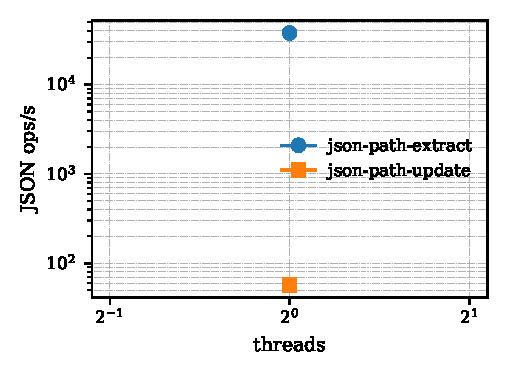
\includegraphics[width=\columnwidth]{figs/fig6_json_throughput.eps}
\caption{JSON path extract and update throughput in the phase-10
cert-v3 lane.}
\label{fig:json}
\end{figure}

\begin{figure}[t]
\centering
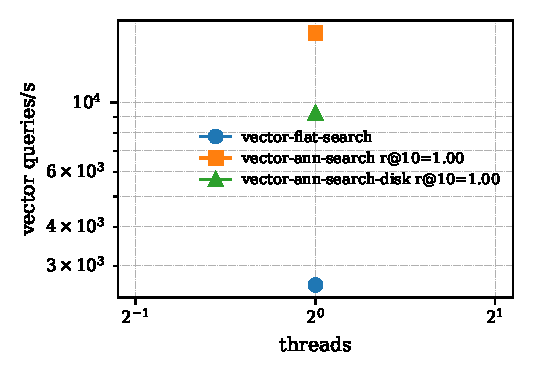
\includegraphics[width=\columnwidth]{figs/fig7_vector_recall_qps.eps}
\caption{Vector search throughput with recall@10 surfaced for ANN
indexes.}
\label{fig:vector}
\end{figure}

\begin{figure}[t]
\centering
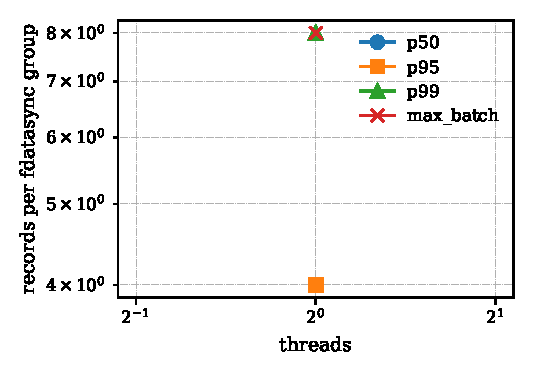
\includegraphics[width=\columnwidth]{figs/fig8_group_commit_batching.eps}
\caption{Group-commit batch-size telemetry under commit-storm load.}
\label{fig:groupcommit}
\end{figure}

\subsection{Telemetry Totals}
Table~\ref{tab:cert} reports the certification totals from
\texttt{paper/data/cert\_totals.csv}.

\begin{table}[t]
\centering
\caption{Certification totals (\texttt{cert\_totals.csv})}
\label{tab:cert}
\renewcommand{\arraystretch}{1.05}
\begin{tabular}{@{}lr@{}}
\toprule
\textbf{Metric} & \textbf{Value} \\
\midrule
Total runs (measured + warmup) & 1{,}728 \\
Measured runs & 1{,}280 \\
Warmup runs (discarded) & 448 \\
Hard failures & 0 \\
Lost acked commits across all scenarios & 0 \\
Recovery matrix passes / total & 36 / 36 \\
Failpoint matrix passes / total & 24 / 24 \\
SQL compatibility passes / total & 40 / 40 \\
Phase-10 workspace tests passing & 691 / 691 \\
Phase-10 active source LOC & 47{,}565 \\
\bottomrule
\end{tabular}
\end{table}

\subsection{Reading the Scaling Curves}
Three patterns are visible across Figs.~\ref{fig:thruput}--\ref{fig:eff}.
First, on the workloads where the SQLite WAL writer is the
bottleneck (the four mixed and writers-disjoint cells), RedlineDB
keeps scaling roughly proportionally to the thread count up to 64
threads, while SQLite saturates near 4--8 threads and the additional
contenders queue. Second, on the read-only workload (point-read-pk),
both engines saturate the host's available memory bandwidth at 64
threads and converge to within 1\%. Third, the 128-thread column
shows the cost of over-subscription on a 128-vCPU host where the
benchmark itself competes with the runtime for cores; throughput
falls for both engines, but RedlineDB's p99 falls less, which
suggests the row-lock manager queues more gracefully than the
SQLite single-writer queue under saturation.

\subsection{Where SQLite Still Wins}
The two losses in Table~\ref{tab:headline} are real. On
\texttt{hot-row-update} (every contender targets a single row),
RedlineDB's row-lock manager serializes every write through one
queue while SQLite's WAL writer batches updates across the same
contention point and amortizes the fsync cost; SQLite's batching wins
this microbenchmark by roughly 5$\times$.
On \texttt{secondary-index-range}, RedlineDB's index cursor lacks
the prefetch path SQLite implements---each leaf chase is a discrete
read where SQLite has already pulled the next page---and the gap is
roughly 80$\times$ at 64 threads. Both losses are addressable by
known engineering work (Section~\ref{sec:discussion}); we report
them rather than excluding them from the matrix.
